\documentclass[tikz]{standalone}
\begin{document}
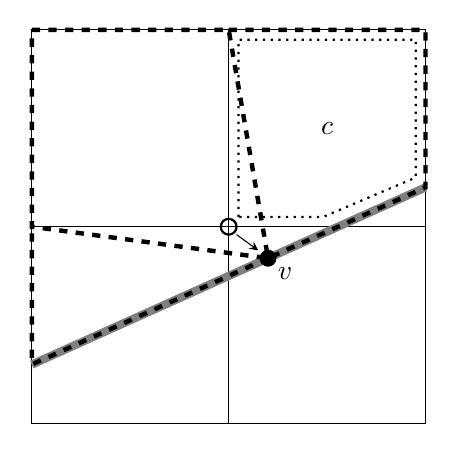
\begin{tikzpicture}[
  scale=0.25
]
\draw (0,0) rectangle (20, 20);
\draw (10,0) -- (10,20);
\draw (0,10) -- (20,10);
\draw [line width=3pt, gray] (0,3) -- (20,12);
\draw [thick, dotted] (10.5,10.5) -- (10.5,19.5) -- (19.5,19.5) -- (19.5,12.5) -- (14.8,10.5) -- (10.5,10.5);
\draw [dashed, ultra thick] (0,20) -- (10,20) -- (12,8.4) -- (0,10) -- (0,20);
\draw [dashed, ultra thick] (12,8.4) -- (0,3) -- (0,10);
\draw [dashed, ultra thick] (10,20) -- (20,20) -- (20,12) -- (12,8.4);
\draw [thick] (10,10) circle [radius=0.4];
\draw [fill=black] (12,8.4) circle [radius=0.4] node [anchor=north west] {$v$};
\draw [->, >=stealth] (10.4,9.6) -- (11.5,8.8);
\node at (15,15) {$c$};
\end{tikzpicture}
\end{document}
